% \Huge

% \todo[inline]{The section names here are just temporary.}

\indent The first step in understanding the evolution of the universe is to look at the theoretical limits we encounter when trying to reconstruct it. As a field is defined at every point in space, any attempt at representing it with data is inherently imperfect. We would have to measure the density field at every point in the Universe in order to obtain all the information it contains. This fact already implies that no data driven reconstruction will ever succeed at perfectly recovering the primordial density field (unless we manage to make an infinity of measurements).

To show this unavoidable loss of information we performed a `perfect' reconstruction. We call this reconstruction `perfect', as it uses data about the primordial positions of all particles (which obviously is not available to observers). However, due to the reasons outlined above, not even this perfect reconstruction succeeds in completely recovering the primordial matter distribution.

\section{Methods}

% \todo[inline]{Present how we did the perfect reconstruction}

The first step in studying reconstruction is to find a way to test its effectiveness. To do this, we use cosmological N-body simulations. These simulations give us important insights into how structure evolves in the Universe. More importantly for this project, it allows us to compare any reconstructed density field to the real starting density field. We use data from three simulations available to us. The first one is Simulation A presented in~\cite{Pontzen_paired_simulations} (also referred to as Simulation A in this work). The other two simulations are variations of the same initial setup, with smaller size and smaller resolution respectively. The details of all three simulations are presented in Table 1.
\todo[inline]{I should probably give a bit more details about the simulations}
\begin{table}[h!]
    \centering
    \begin{tabular}{ |c|c|c|c| } 
        \hline
        Label & Size & Number of Particles & Particle Mass (Solar Masses) \\
        \hline
        Sim A & $(200 Mpc)^3$ & $512^3$ & $6.59 \times 10^9$ \\ 
        \hline
        Sim B & $(200 Mpc)^3$ & $256^3$ & $5.27 \times 10^{10}$ \\ 
        \hline
        Sim C & $(100 Mpc)^3$ & $256^3$ & $6.59 \times 10^9$ \\ 
        \hline
        
    \end{tabular}
    \caption{The sizes and number of particles of the three simulations used in this project.}
    \label{table:1}
\end{table}

% \cite{Eisenstein_BAOpeak_reconstruction}

The idea behind a perfect reconstruction is to use data about the initial state of the simulation to perform the reconstruction. We have access to multiple snapshots at various redshifts in our simulations, including the initial positions of all particles (at $z = 99$). Therefore, we used this information to reconstruct the density field. We first measured the density field of various snapshots in the redshift interval $z = 0 - 9$. The field was measured at the particle positions instead of being measured on a regular grid. This is because we want the particles to carry the density field when we move them. After that, all the particles were moved to their starting positions (taken from the initial snapshot at $z = 99$).




\section{From Images to Statistics}

% \todo[inline]{Show some density slices of the results, and talk about the effects that pop up (e.g. the increase in total mass). Show Power Spectra}

\subsection{The Reconstructed Density Field}

As outlined above, the first step is to measure the density field in a snapshot. Each snapshot contains an indexed list with the positions, velocities and masses of all particles in the simulation. In this chapter, only the positions and masses are needed to perform a perfect reconstruction. To perform the first part of this analysis, we used the \textit{pynbody}\footnote{https://github.com/pynbody/pynbody} package (\cite{2013ascl.soft05002P}). 

To have a visual understanding of the reconstruction, we first make some images of the density field. We use \textit{pynbody} to import the initial snapshot and the snapshot at $z=0$. The density field at the particle locations in the final snapshot is calculated and assigned as the density field of the initial snapshot. Density slices through this reconstructed field are compared to the initial and final fields in Figure \todo{put image in and ref}. 

We can already see from this comparison that the reconstruction has not recovered all the information, as it is not identical to the initial filed. However, we see the effect that we are after. The reconstruction spreads out the matter from the collapsed filaments onto a more uniform field. Also notice the large difference in the values of the density field. The reconstructed field has density values about 3 orders of magnitude larger than the initial field. \todo{also talk about the density distribution}

This large difference is an interesting side effect of our method. At late times, most particles tend to be clumped together. Therefore, when measuring the density field at the particle positions, we will mostly get very high values. These values do not change when moving the particles, so the final field will also have very high values, but this time distributed on an almost uniform grid. This results in an apparent increase in the total mass of the simulation. As this increase is just a result of the way we represent the density field, it needs to be accounted for when analysing the results. The total mass of the simulation should be conserved.

\subsection{Correlation with the Initial Field}

\todo[inline]{TALK ABOUT TAKING THE LOG OF THE DENSITY FIELD}

In order to get a better understanding of how well this reconstruction worked, we turn to statistics. A good way to represent the reconstruction  is to look at the normalized Cross-Spectrum between the initial and the reconstructed field: $$ \frac{P_{IX}(k)}{\sqrt{P_I(k) * P_X(k)}} $$ where $I$ represents the initial field, and $X$ the reconstructed field. \todo{The power-spectrum will be introduced in chapter 2}

We used the \textsc{GenPK} code\footnote{https://github.com/sbird/GenPK.git} (\cite{2017ascl.soft06006B}) to measure auto and cross power-spectra of \textsc{Gadget} outputs. The original normalized cross-spectra between the initial and the final fields (from Sim A) can be seen in Figure \ref{fig:3.1}. For small wavenumbers $k$ (corresponding to large scales), the correlation is very good (converges to 1: perfect correlation). On the other hand, for large wavenumbers (corresponding to small scales), the two fields are completely decorrelated. 
\todo[inline]{Talk about the binning??}

\begin{figure}
    \centering
    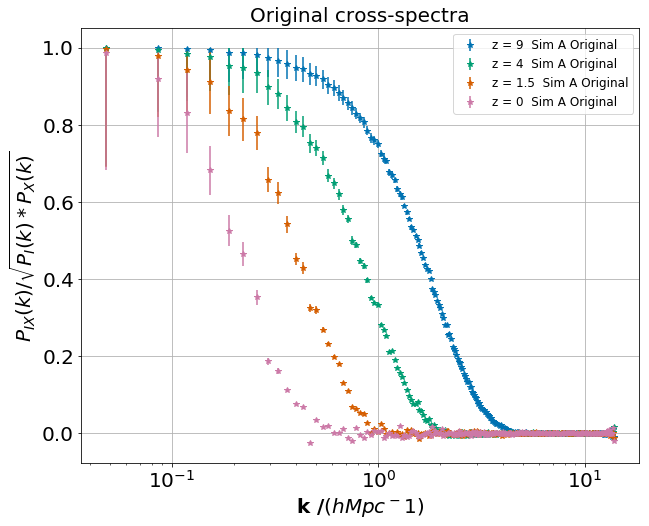
\includegraphics[width=1\columnwidth]{images/perfRecon/orig.png}%
    
    \caption{
    Normalized cross-spectra between the initial and final density fields as a function of scale. At small wavenumbers $k$ (large scales) the two fields are perfectly correlated because the universe is not affected by gravitational collapse over such scales (they are both uniform). On the other hand, at large $k$ (small scales) they are decorrelated because the initial field is very uniform, while the final field is very non-uniform on such scales (it contains large empty voids, and small and massive halos). The decorrelation scale moves to smaller $k$ as time goes on due to the progressive collapse of larger and larger overdensities.
    }
    
    \label{fig:3.1}
\end{figure}

The small $k$ convergence towards perfect correlation indicates that gravitational collapse does not have a large impact over such large scales. Because of this, both the initial and the final density fields tend to be very uniform, which preserves the correlation on these scales. However, over small scales, gravity has a large impact. This results in a large discrepancy between massive collapsed regions and mostly empty voids. This is in stark contrast to the relative uniformity of the initial field, leading to breakdown in correlation.

Figure \ref{fig:3.1} also shows the evolution of this correlation with redshift. The wavenumber at which the two fields decorrelate indicates the progress of gravitational collapse at that redshift. This results in the decorrelation scale moving to smaller wavenumbers with the progress of gravitational collapse. The objective of reconstruction methods is to bring this decorrelation scale to larger $k$ (in order to recover information about the initial field).

\todo[inline]{Talk about errors here}

In order to measure the power-spectra of our reconstructed fields, we modified \textsc{GenPK} to read the fields generated by \textit{pynbody}. The results of the perfect reconstruction can be seen in Figure \ref{fig:3.2}, where we compare it with the original correlation at different redshifts. 

\begin{figure}
    \centering
    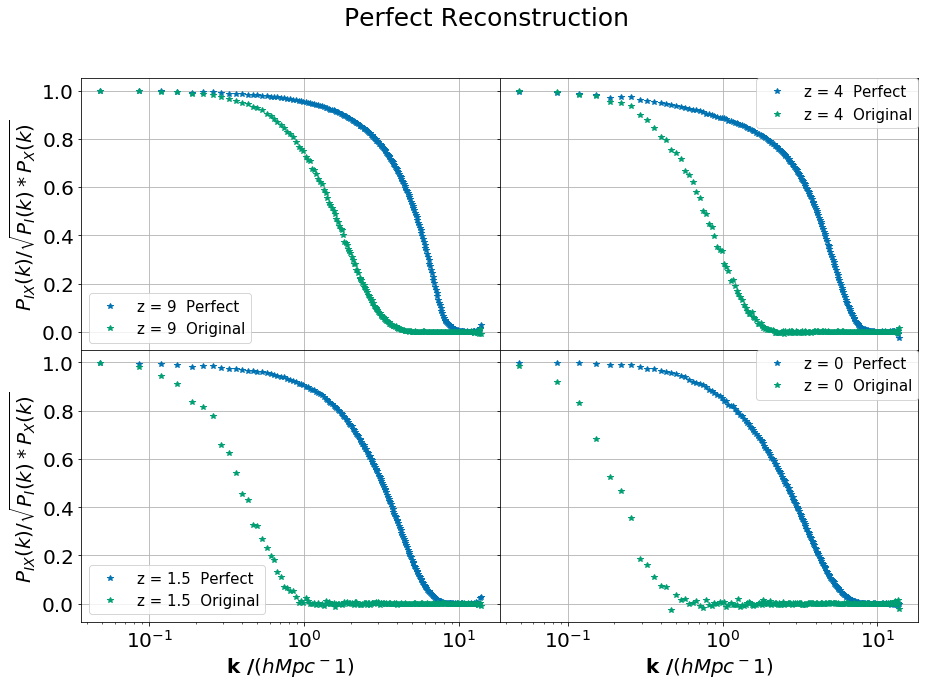
\includegraphics[width=1\columnwidth]{images/perfRecon/perfRecon.png}%
    
    \caption{
    Normalized cross-spectra between the initial and the reconstructed fields compared to the original correlation. A large improvement in the correlation was achieved with the perfect reconstruction. This shows up as a shift of the decorrelation scale towards larger $k$ (smaller scales). However, the perfect reconstruction does not lead to a perfect correlation due to the limiting resolution of our density field measurements. When comparing the reconstruction applied to fields at different redshift, we see a trend towards more information being recovered from smaller redshifts.
    }
    
    \label{fig:3.2}
\end{figure}

\section{Analysis}

The cross-spectra presented in Figure~\ref{fig:3.2} show a large improvement in the correlation with the initial field. There is also an increase in the amount of information recovered for lower redshifts. This means redshift does not play a role as large in the perfect reconstruction as it originally did. 

\begin{figure}
    \centering
    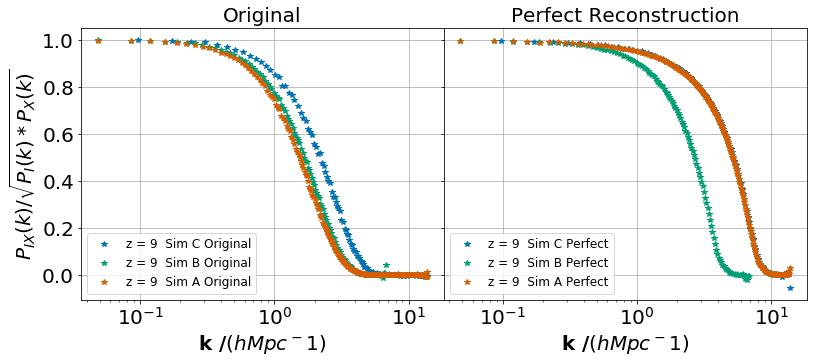
\includegraphics[width=1\columnwidth]{images/perfRecon/simComp.png}%
    
    \caption{
    Normalized cross-spectra across the three simulations. The left plot shows the original correlation between the initial and the final fields, and the right panel shows the correlation with the reconstructed field. For the original correlations, the size of the simulation plays an important role, with the smaller simulation decorrelating on smaller scales. However, after the reconstruction, the size of the simulation does not seem to have any impact (with Sim A being almost identical to Sim C). In this case, the resolution of the simulation is the only factor that matters, with the larger resolution simulations showing a better correlation.
    }
    
    \label{fig:3.3}
\end{figure}
However, in order to understand this perfect reconstruction, we need to look at the key role played by the resolution of the simulation. Figure~\ref{fig:3.3} shows a comparison of the cross-spectra across the three simulations. For the original correlations, the size of the simulation plays a larger role than the resolution. Simulation C (smaller size) shows a smaller scale of decorrelation. Simulations A and B (same size) are very close, with a slight edge for simulation B (lower resolution). \todo{better explination here}

A completely different structure can be seen once we perform the perfect reconstruction. Simulation A and C (same resolution) show identical reconstructed correlation, while the reconstruction in Simulation B (lower resolution) does not perform as well. This indicates that resolution plays the decisive role in the perfect reconstruction. However, this was exactly the starting point of this chapter. The limiting factor for this reconstruction is the resolution used to measure the density field. The right panel in Figure~\ref{fig:3.3} shows the lowest scale that can be reconstructed depending on the resolution of our simulation.

The perfect reconstructions in Figure~\ref{fig:3.2} show that a perfect correlation cannot be achieved even in the ideal case of perfect knowledge of all the starting particle positions. However, a large improvement in the correlation can be seen, with the decorrelation scale moving to very small scales (of the order $1 Mpc$). This ideal reconstruction using perfect knowledge of the particle positions serves as a theoretical upper limit to reconstruction techniques. The perfect reconstruction, along with the original correlation, will always be present in the next chapter when we look at realistic reconstructions. This can give us a better understanding to how well our techniques work.


% \begin{figure}
%     \centering
%     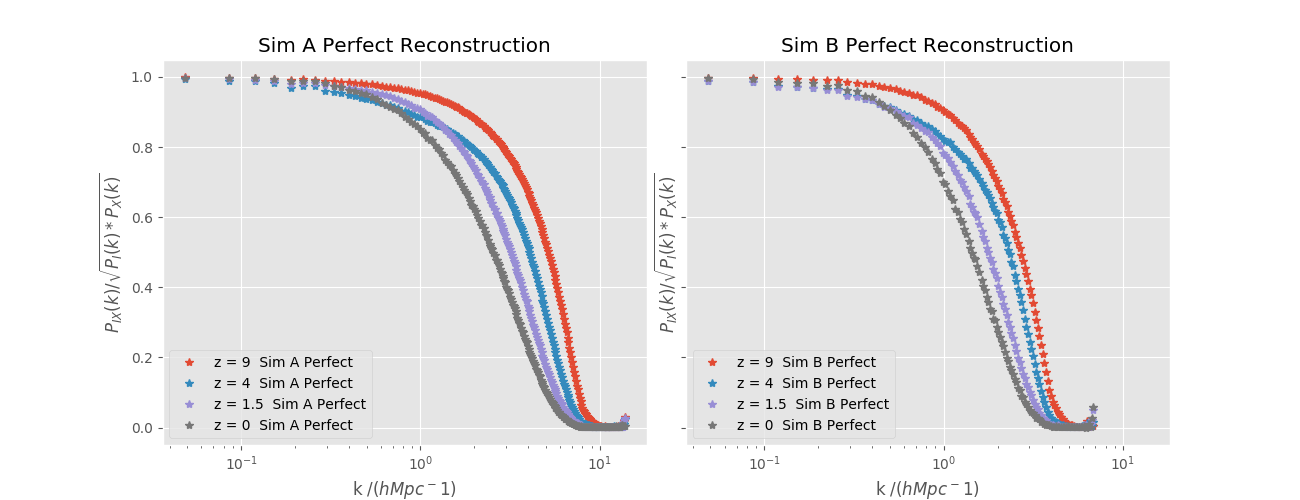
\includegraphics[width=1\columnwidth]{images/crossSpectra/Spec_3_perf.png}%
    
%     \caption{
%     Perfect Reconstruction from different redshifts in Sim A and Sim B
%     }
    
%     \label{fig:6}
% \end{figure}